\begin{savequote}[75mm]
Q: Why did the chicken cross the road?

A: The answer is trivial and is left as an exercise for the reader.
%\qauthor{--- Queen Elizabeth II ---}
\end{savequote}

\chapter{Three-dimensional analytical geometry}
\label{chap_ana_geo}
\graphicspath{{figures/Ana_Geo/}}

In Chapter~\ref{chap_vector} we already introduced Cartesian coordinates in space when discussing vectors in space. Of course, we can make use of that framework to extend also analytical geometry to three dimensions. We start our brief discussion with lines and planes, after which we turn to more involved objects such as quadratic surfaces. 

\section{Lines}\label{sec:lines}
\subsection{Definition}
\ifcourse
	\checkoddpage
\marginpar{\ifoddpage\hspace*{-1.5cm}\else\hspace*{0.25cm}\fi\includegraphics[width=0.075\textwidth]{youtube}\\
\ifoddpage\hspace*{-1.75cm}\else\hspace*{0.1cm}\fi
\qrcode[height=1.75cm]{https://www.brightstorm.com/math/precalculus/vectors-and-parametric-equations/lines-in-3d/}
%\includegraphics[width=0.1\textwidth]{lines_3d}
}
 \fi
To find the equation of \textbf{a line} (\textit{rechte}) in the $xy$-plane, we need a point on the line and the direction of the line. This also holds true for lines in space. Let $P$ be a point in space, let $\vec p$ be the vector with initial point at the origin and terminal point at $P$ (i.e., $\vec p$ points to $P$), and let $\vec d$ be a vector. Consider the points on the line through $P$ in the direction of $\vec d$. Clearly one point on the line is $P$; we can say that the vector $\vec p$ lies at this point on the line. To find another point on the line, we can start at $\vec p$ and move in a  direction parallel to $\vec d$. For instance, starting at $\vec p$ and travelling one length of $\vec d$ places one at another point on the line. Consider Figure \ref{fig_ana_geo_1} where certain points along the line are indicated. The figure illustrates how every point on the line can be obtained by starting with $\vec p$ and moving a certain distance in the direction of $\vec d$. That is, we can define the line as a function of $t$ using a \textbf{vector equation} (\textit{vectorvergelijking van een rechte}):
\index[aut]{vectorvergelijking van een rechte} \index{vector equation}
\begin{equation}\vec\ell(t) = \vec p + t\ \vec d.\label{eq:lines1}\end{equation}


\begin{figure}
	\begin{center}
			\includegraphics[width=0.5\textwidth]{fig_ana_geo_1}
	\caption{Defining a line in space.}
	\label{fig_ana_geo_1}
	\end{center}
\end{figure}

In many ways, this is not a new concept. Compare Equation \eqref{eq:lines1} to the familiar $y=mx+b$ equation of a line:
\usetikzlibrary{calc}
\begin{center}
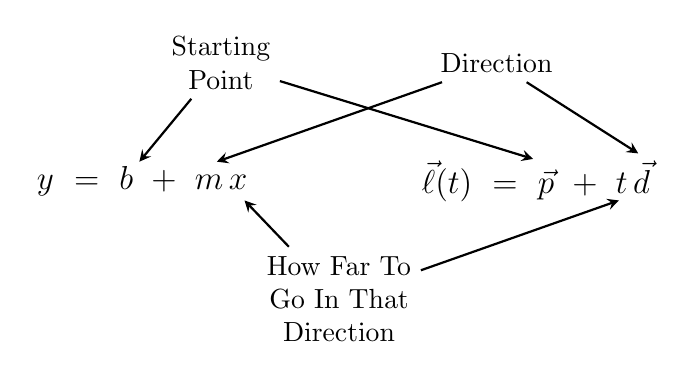
\begin{tikzpicture}[>=stealth]
	\draw (0,0) node (L) {\large $y\ =\ b\ +\ m\,x$};
	\draw (5,0) node (R) {\large $\vec \ell(t)\ =\ \vec p\ +\ t\,\vec d$};
\node (A) at (1,1.5) [align=center,] {Starting\\ Point};
\node (B) at (4.5,1.5) [align=center] {Direction};
\node (C) at (2.5,-1.5) [align=center] {How Far To\\  Go In That \\Direction};
\draw [->,thick] (A) -- ($(R)+(-1pt,8pt)$);	
\draw [->,thick] (A) -- ($(L)+(-1pt,7pt)$);
\draw [->,thick] (B) -- ($(L)+(27pt,7pt)$);%(.9,.2);
\draw [->,thick] (B) -- ($(R)+(37pt,10pt)$);
\draw [->,thick] (C) -- ($(L)+(37pt,-7pt)$);%(1.3,-.15);
\draw [->,thick] (C) -- ($(R)+(30pt,-7pt)$);
\end{tikzpicture}
\captionsetup{type=figure}%
\caption{Understanding the vector equation of a line.}
\label{fig:lines_eq}
\end{center}

The equations exhibit the same structure: they give a starting point, define a direction, and state how far in that direction to travel.

Equation~\eqref{eq:lines1} is an example of a \textbf{vector--valued function} (\textit{vectorfunctie}); the input of the function is a real number and the output is a vector. We will cover vector--valued functions extensively in Chapter~\ref{chap_vector_fun}.
\index[aut]{vectorfunctie} \index{vector--valued function}

There are other ways to represent a line. Let $\vec p = ( x_0,y_0,z_0)$ and let $\vec d = ( a,b,c)$. Then the equation of the line through $\vec p$ in the direction of $\vec d$ is:
\begin{align*}
\vec\ell(t) &= \vec p + t\,\vec d \\
						&= ( x_0,y_0,z_0) + t( a,b,c) \\
						&= ( x_0 + at, y_0+bt, z_0+ct).
\end{align*}

The last line states that the $x$-values of the line are given by $x=x_0+at$, the $y$-values are given by $y = y_0+bt$, and the $z$-values are given by $z = z_0 + ct$. These three equations, taken together, are the \textbf{parametric equations of the line} (\textit{parametervoorstelling van een rechte}) through $\vec p$ in the direction of $\vec d$.
\index{parametric equations of the line} \index[aut]{parametervoorstelling van een rechte}

Finally, each of the equations for $x$, $y$ and $z$ above contain the variable $t$:
$$
\left\{
\begin{array}{lcl}
x &=& x_0+at,\\
y&=&y_0+bt, \\
z &=& z_0+ct.\\
\end{array}
\right.
$$

We can solve for $t$ in each equation to obtain:
\renewcommand{\arraystretch}{2}
$$
\left\{
\begin{array}{lcl}
 t&=&\dfrac{x-x_0}{a},\\
 t &=& \dfrac{y-y_0}{b},\\
 t &=& \dfrac{z-z_0}{c}.\\
\end{array}
\right.
$$
\renewcommand{\arraystretch}{1}

assuming $a,b,c\neq 0$.
Since $t$ is equal to each expression on the right, we can set these equal to each other, forming the \textbf{Cartesian equations of the line} (\textit{cartesische vergelijkingen van een rechte}) through $\vec p$ in the direction of $\vec d$:
$$\frac{x-x_0}{a} = \frac{y-y_0}{b}=\frac{z-z_0}{c}.$$
Each representation has its own advantages, depending on the context. We summarize these three forms in the following definition, then give examples of their use.
\index{symmetric equations of the line} \index[aut]{cartesische vergelijkingen van een rechte}

\begin{definition}[Equations of lines in space]\label{def:lines}
Consider the line in space that passes through $\vec p = (x_0,y_0,z_0)$ in the direction of $\vec d = ( a,b,c).$
\begin{enumerate}[align=left]
	\item The \textbf{vector equation} of the line is $$\vec \ell(t) = \vec p+t\vec d.$$
	\item The \textbf{parametric equations} of the line are
	$$
\left\{
\begin{array}{lcl}
x &=& x_0+at,\\
y&=&y_0+bt, \\
z &=& z_0+ct.\\
\end{array}
\right.
$$

	\item The \textbf{symmetric equations} of the line are
	$$\frac{x-x_0}{a} = \frac{y-y_0}{b}=\frac{z-z_0}{c}.$$
\end{enumerate}
\end{definition}

\begin{example}\label{ex_lines1}
Give all three equations, as given in Definition \ref{def:lines}, of the line through $P = (2,3,1)$ in the direction of $\vec d = ( -1,1,2)$.

\xhrulefill{gray}{2.5pt}Solution \xhrulefill{gray}{2.5pt}

We identify the point $P=(2,3,1)$ with the vector $\vec p =( 2,3,1)$. Following the definition, we have
\begin{itemize}
	\item the vector equation of the line is $\vec\ell(t) = ( 2,3,1) + t( -1,1,2)$;
	\item	the parametric equations of the line are
		$$
\left\{
\begin{array}{lcl}
x &=& 2-t,\\
y&=&3+t, \\
z &=& 1+2t;\\
\end{array}
\right.
$$
and
	\item	the symmetric equations of the line are
	$$\frac{x-2}{-1}=\frac{y-3}{1} = \frac{z-1}{2}.$$
\end{itemize}

The resulting line is graphed in Figure~\ref{fig_ana_geo_2}.

\begin{figure}[H]
	\begin{center}
			\includegraphics[width=0.4\textwidth]{fig_ana_geo_2}
	\caption{Graphing the line from Example \ref{ex_lines1}.}
	\label{fig_ana_geo_2}
	\end{center}
\end{figure}


The first two equations of the line are useful when a $t$ value is given: one can immediately find the corresponding point on the line. These forms are good when calculating with a computer; most software programs easily handle equations in these formats. 
\end{example}

\subsection{Relative position of lines}

In the plane, two distinct lines can either be parallel or they will intersect at exactly one point. In space, given the equations of two lines, it can sometimes be difficult to tell whether the lines are distinct or not (i.e., the same line can be represented in different ways). Given lines $\vec\ell_1(t) = \vec p_1 + t\vec d_1$ and $\vec \ell_2(t) = \vec p_2+t\vec d_2$, we have four possibilities: $\vec \ell_1$ and $\vec \ell_2$ are
\index{lines!skew}\index{lines!parallel}\index{lines!intersecting}

\renewcommand{\arraystretch}{1.5}
\begin{center}
\begin{tabular}{p{200pt}p{150pt}}
the \textbf{same line} (\textit{samenvallend}) & they share all points; \\
\textbf{intersecting} (\textit{snijdend}) lines & share only 1 point;\\
\textbf{parallel} (\textit{evenwijdig}) lines & $\vec d_1\parallel \vec d_2$, no points in common; \\
\textbf{skew} (\textit{kruisend}) lines & $\vec d_1 \not\parallel \vec d_2$, no points in common. 
\index[aut]{samenvallend} \index[aut]{snijdend} \index[aut]{evenwijdig} \index{same line} \index{intersecting} \index {parallel}
\end{tabular}
\end{center}
\renewcommand{\arraystretch}{1}


\pagebreak
\begin{example}\label{ex_lines2}
Consider lines $\ell_1$ and $\ell_2$, given in parametric equation form

$$\ell_1: \left\{\begin{array}{ccl} x&=&1+3t \\ y&=&2-t\\z&=&t\end{array}\right.\qquad\text{and}\qquad \ell_2: \left\{\begin{array}{ccl} x&=&-2+4s\\y&=&3+s\\z&=&5+2s\,.\end{array}\right.
$$

%\ell_1:\; \begin{cases} x&=1+3t \\ y&=2-t\\z&=t\end{cases}\qquad\qquad\qquad
%\ell_2:\; \begin{cases} x&=-2+4s\\y&=3+s\\z&=5+2s\,.\end{cases}
%$$


Determine whether $\ell_1$ and $\ell_2$ are the same line, intersect, are parallel, or skew.

\xhrulefill{gray}{2.5pt}Solution \xhrulefill{gray}{2.5pt}

We start by looking at the directions of each line. Line $\ell_1$ has the direction given by $\vec d_1=( 3,-1,1)$ and line $\ell_2$ has the direction given by $\vec d_2 = ( 4,1,2)$. It should be clear that $\vec d_1$ and $\vec d_2$ are not parallel, hence $\ell_1$ and $\ell_2$ are not the same line, nor are they parallel. Figure \ref{fig_ana_geo_3} verifies this fact. It shows the points and directions indicated by the equations of each line are identified.


\begin{figure}[H]
	\begin{center}
			\includegraphics[width=0.35\textwidth]{fig_ana_geo_3}
	\caption{Sketching the lines from Example \ref{ex_lines2}.}
	\label{fig_ana_geo_3}
	\end{center}
\end{figure}


We next check to see if they intersect (if they do not, they are skew lines). To find if they intersect, we look for $t$ and $s$ values such that the respective $x$, $y$ and $z$ values are the same. That is, we want $s$ and $t$ such that:
$$\left\{
\begin{array}{rcl}
1+3t &=&-2+4s\\
2-t&=&3+s\\
t&=&5+2s\,.\end{array}
\right.$$
This is a relatively simple system of linear equations. Since the last equation is already solved for $t$, we substitute that value of $t$ into the equation above it:
$$2-(5+2s) = 3+s \quad \Rightarrow \quad s=-2,\quad t=1\,.$$
A key to remember is that we have three equations; we need to check if $s=-2,\, t=1$ satisfies the first equation as well:
$$1+3(1) \neq -2+4(-2).$$
It does not. Therefore, we conclude that the lines $\ell_1$ and $\ell_2$ are skew.
\end{example}

%\subsection{Distances to lines}
%
%Given a point $Q$ and a line $\vec\ell(t) = \vec p+t\vec d$ in space, it is often useful to know the distance from the point to the line.  Identifying $\vec p$ with the point $P$, Figure~\ref{fig_ana_geo_4a} will help establish a general method of computing this distance $h$.
%
%
%\begin{figure}[H]
%\centering
%%)isebox{0.5cm}{
%\centerline{
%\subfigure[\label{fig_ana_geo_4a}]{\includegraphics[width=0.35\textwidth]{fig_ana_geo_4a}}
%\hspace{0.1cm}
%\subfigure[\label{fig_ana_geo_4b}]{\includegraphics[width=0.35\textwidth]{fig_ana_geo_4b}}
%}
%\caption{Establishing the distance from a point to a line (a) and between lines (b). }
%\end{figure}
%
%
%From trigonometry, we know $h = \norm{\vv{PQ}}\sin(\theta)$. We have a similar identity involving the cross product: $\norm{\vv{PQ}\times \vec d} = \norm{\vv{PQ}}\, \vnorm{d}\sin(\theta).$ Dividing both sides of the latter equation by $\vnorm{d}$ yields $h$:
%\begin{equation}
%h = \frac{\norm{\vv{PQ}\times \vec d}}{\vnorm{d}}.
%\label{eq:lines2}
%\end{equation}
%
%
%
%
%It is also useful to determine the distance between lines, which we define as the length of the shortest line segment that connects the two lines. Let lines $\vec\ell_1(t) = \vec p_1 + t\vec d_1$ and $\vec\ell_2(t) = \vec p_2 + t\vec d_2$ be given, as shown in Figure \ref{fig_ana_geo_4b}. To find the direction orthogonal to both $\vec d_1$ and $\vec d_2$, we take the cross product: $\vec c = \vec d_1\times \vec d_2$. The magnitude of the orthogonal projection of $\vv{P_1P_2}$ onto $\vec c$ is the distance $h$ we seek:
%
%\begin{eqnarray}
%h&=&		\snorm{\text{proj}\,_{\vec c}\,\vv{P_1P_2}}\nonumber\\
%	&=& \snorm{\frac{\vv{P_1P_2}\cdot\vec c}{\dotp cc}\vec c}\nonumber\\
%	&=&\frac{|\vv{P_1P_2}\cdot \vec c|}{\vnorm c^2}\vnorm c\nonumber\\
%	&=&\frac{|\vv{P_1P_2}\cdot \vec c|}{\vnorm c} \label{eq:lines3}.
%\end{eqnarray}
% Note the use of the triple scalar product: $\vv{P_1P_2}\cdot \vec c = \vv{P_1P_2}\cdot (\vec d_1\times \vec d_2).$
%
%\begin{example}\label{ex_lines4}
%Find the distance from the point $Q=(1,1,3)$ to the line $\vec\ell(t) = ( 1,-1,1)+t( 2,3,1).$
%
%\xhrulefill{gray}{2.5pt}Solution \xhrulefill{gray}{2.5pt}
%
%The equation of the line gives us the point $P=(1,-1,1)$ that lies on the line, hence $\vv{PQ} = ( 0,2,2)$. The equation also gives $\vec d= ( 2,3,1)$. Following Equation~\eqref{eq:lines2}, we have the distance as 
%\begin{align*}
%h &= \frac{\norm{\vv{PQ}\times \vec d}}{\vnorm{d}}\\
%	&= \frac{\norm{( -4,4,-4)}}{\sqrt{14}}\\
%	&=\frac{4\sqrt{3}}{\sqrt{14}} \approx 1.852.
%\end{align*}
%The point $Q$ is approximately $1.852$ units from the line $\vec\ell(t)$.
%\end{example}
%
%\begin{example}\label{ex_lines5}
%Find the distance between the lines 
%$$\ell_1: \left\{\begin{array}{ccl} x&=&1+3t \\ y&=&2-t\\z&=&t\end{array}\right.\qquad\text{and}\qquad \ell_2:\left\{\begin{array}{ccl} x&=&-2+4s\\y&=&3+s\\z&=&5+2s.\end{array}\right.$$
%
%\xhrulefill{gray}{2.5pt}Solution \xhrulefill{gray}{2.5pt}
%
%These are the same lines as given in Example \ref{ex_lines2}, where we showed them to be skew. The equations allow us to identify the following points and vectors:
%$$P_1 = (1,2,0)\quad P_2 = (-2,3,5) \quad \Rightarrow \quad \vv{P_1P_2} = ( -3,1,5).$$
%$$\vec d_1 = ( 3,-1,1) \quad \vec d_2 = ( 4,1,2) \quad \Rightarrow \quad \vec c = \vec d_1\times \vec d_2 = ( -3,-2,7).$$
%From Equation~\eqref{eq:lines3} we have that the distance $h$ between the two lines is
%\begin{align*}
%h &= \frac{|\vv{P_1P_2}\cdot \vec c|}{\vnorm c}\\
%&=\frac{42}{\sqrt{62}} \approx 5.334.
%\end{align*}
%The lines are approximately 5.334 units apart.
%\end{example}

One of the key points to understand from this section is this: to describe a line, we need a point and a direction. Lines are one of two fundamental objects of study in space. The other fundamental object is the plane, which we study in detail in the next section. Many complex three dimensional objects are studied by approximating their surfaces with lines and planes.


\section{Planes}\label{sec:planes}
\subsection{Definition}
\ifcourse
	\checkoddpage
\marginpar{\ifoddpage\hspace*{-1.5cm}\else\hspace*{0.25cm}\fi\includegraphics[width=0.075\textwidth]{youtube}\\
\ifoddpage\hspace*{-1.75cm}\else\hspace*{0.1cm}\fi
\qrcode[height=1.75cm]{https://www.brightstorm.com/math/precalculus/vectors-and-parametric-equations/vectors-and-planes/}
%\includegraphics[width=0.1\textwidth]{planes_3d}
}
 \fi
Any flat surface, such as a wall, table top or stiff piece of cardboard can be thought of as representing part of a \textbf{plane} (\textit{vlak}). Consider a piece of cardboard with a point $P$ marked on it. One can take a nail and stick it into the cardboard at $P$ such that the nail is perpendicular to the cardboard. This nail provides a handle for the cardboard. Moving the cardboard around moves $P$ to different locations in space. Tilting the nail but keeping $P$ fixed tilts the cardboard. Both moving and tilting the cardboard defines a different plane in space. In fact, we can define a plane by: 1) the location of $P$ in space, and 2) the direction of the nail.
\index{plane} \index[aut]{vlak}

The previous section showed that one can define a line given a point on the line and the direction of the line. One can make a similar statement about planes: we can define a plane in space given a point on the plane and the direction the plane faces. Once again, the direction information will be supplied by a vector, called a \textbf{normal vector} (\textit{normaalvector}), that is orthogonal to the plane.
\index{vectors!normal vector}\index{normal vector}\index{planes!normal vector}\index[aut]{normaal}\index[aut]{vlak ! normaal}

What exactly does orthogonal to the plane mean? Choose any two points $P$ and $Q$ in the plane, and consider the vector $\vv{PQ}$. We say a vector $\vec n$ is orthogonal to the plane if $\vec n$ is perpendicular to $\vv{PQ}$ for all choices of $P$ and $Q$; that is, if $\vec n\cdot \vv{PQ}=0$ for all $P$ and $Q$. This gives us way of writing an equation describing the plane. Let $P=(x_0,y_0,z_0)$ be a point in the plane and let $\vec n = ( a,b,c) $ be a normal vector to the plane. A point $Q = (x,y,z)$ lies in the plane defined by $P$ and $\vec n$ if and only if, $\vv{PQ}$ is orthogonal to $\vec n$. Knowing $\vv{PQ} = ( x-x_0,y-y_0,z-z_0)$, consider:
\begin{align}
\vv{PQ}\cdot\vec n &= 0 \notag\\
				\Leftrightarrow\quad\;\;\, ( x-x_0,y-y_0,z-z_0)\cdot ( a,b,c) &=0\notag\\
				\Leftrightarrow\quad a(x-x_0)+b(y-y_0)+c(z-z_0) &=0. \label{eq:planes1}
\intertext{Equation \eqref{eq:planes1} defines an implicit function describing the plane. More algebra produces:}
ax+by+cz &= ax_0+by_0+cz_0. \notag
\intertext{The right hand side is just a number, so we replace it with $d$:}
ax+by+cz &= d\label{eq:planes2}.
\end{align}
As long as $c\neq 0$, we can solve for $z$:
\begin{equation}
z = \frac1c(d-ax-by).\label{eq:planes3}
\end{equation}
 Equation \eqref{eq:planes3} is especially useful as many computer programs can graph functions in this form. Equations \eqref{eq:planes1} and \eqref{eq:planes2} have specific names, given next.

\begin{definition}[Equations of a plane]\label{def:planes}
The \textbf{plane} passing through the point $P=(x_0,y_0,z_0)$ with normal vector $\vec n=( a,b,c)$ can be described by an \textbf{equation with standard form} $$a(x-x_0)+b(y-y_0)+c(z-z_0) =0;$$
the equation's general form is 
\index{planes!equations of}
$$ax+by+cz = d.$$
\end{definition}

Clearly, the coordinate axes naturally define three planes (shown in Figure \ref{fig_ana_geo_4}), the \textbf{coordinate planes} (\textit{co\"ordinaatvlak}): the $xy$-plane, the $yz$-plane and the $xz$-plane. The $xy$-plane is characterized as the set of all points in space where the $z$-value is 0. %(Likewise, the $xz$-plane is all points where the $y$-value is 0.) 
\index{planes!coordinate plane}\index[aut]{co\"ordinaatvlak}
This, in fact, gives us an equation that describes this plane: $z=0$. Likewise, the $xz$-plane is all points where the $y$-value is 0, characterized by $y=0$. Furthermore, the equation $x=2$ describes all points in space where the $x$-value is 2.




A key to remember throughout this section is this: to find the equation of a plane, we need a point and a normal vector. We will give several examples of finding the equation of a plane, and in each one different types of information are given. In each case, we need to use the given information to find a point on the plane and a normal vector.

\begin{figure}[H]
\centering
%)isebox{0.5cm}{
\centerline{
\subfigure[The $xy$-plane. \label{fig_ana_geo_4a}]{\includegraphics[width=0.3\textwidth]{fig_ana_geo_4a}}
\hspace{0.1cm}
\subfigure[The $yz$-plane. \label{fig_ana_geo_4b}]{\includegraphics[width=0.3\textwidth]{fig_ana_geo_4b}}
\hspace{0.1cm}
\subfigure[The $xz$-plane. \label{fig_ana_geo_4c}]{\includegraphics[width=0.3\textwidth]{fig_ana_geo_4c}}
}
\caption{The coordinate planes. }
\label{fig_ana_geo_4}
\end{figure}


\begin{example}\label{ex_planes1}
Write the equation of the plane that passes through the points $P=(1,1,0)$, $Q = (1,2,-1)$ and $R = (0,1,2)$ in standard form.

\xhrulefill{gray}{2.5pt}Solution \xhrulefill{gray}{2.5pt}

We need a vector $\vec n$ that is orthogonal to the plane. Since $P$, $Q$ and $R$ are in the plane, so are the vectors $\vv{PQ}$ and $\vv{PR}$; $\vv{PQ}\times\vv{PR}$ is orthogonal to $\vv{PQ}$ and $\vv{PR}$ and hence the plane itself.

It is straightforward to compute $\vec n = \vv{PQ}\times\vv{PR} = ( 2,1,1)$. We can use any point we wish in the plane (any of $P$, $Q$ or $R$ will do) and we arbitrarily choose $P$. Following Definition \ref{def:planes}, the equation of the plane in standard form is 
$$2(x-1) + (y-1)+z = 0.$$
The plane is sketched in Figure \ref{fig_ana_geo_5}.


\begin{figure}[H]
	\begin{center}
			\includegraphics[width=0.3\textwidth]{fig_ana_geo_5}
	\caption{Sketching the plane in Example \ref{ex_planes1}.}
	\label{fig_ana_geo_5}
	\end{center}
\end{figure}

\end{example}

We have just demonstrated the fact that any three non-collinear points define a plane. This is why a three-legged stool does not rock; its three feet always lie in a plane. A four-legged stool will rock unless all four feet lie in the same plane.


\begin{example}\label{ex_planes2}
Verify that lines $\ell_1$ and $\ell_2$, whose parametric equations are given below, intersect, then give the equation of the  plane that contains these two lines in general form.
$$ \ell_1: \left\{\begin{array}{lcl} x&=&-5+2s \\ y&=&1+s \\ z&=&-4+2s\end{array}\right. \qquad\qquad\qquad
				\ell_2: \left\{\begin{array}{lcl} x &=& 2+3t\\ y&=&1-2t \\ z&=&1+t\end{array}\right.$$

\xhrulefill{gray}{2.5pt}Solution \xhrulefill{gray}{2.5pt}


The lines clearly are not parallel. If they do not intersect, they are skew, meaning there is not a plane that contains them both. If they do intersect, there is such a plane. 

To find their point of intersection, we set the $x$, $y$ and $z$ equations equal to each other and solve for $s$ and $t$:
$$\left\{\begin{array}{lcl}
-5+2s &=&2+3t \\ 1+s &=& 1-2t \\ -4+2s &=& 1+t \end{array}\right.\quad  \Rightarrow  \quad s=2,\quad t=-1.$$

When $s=2$ and $t=-1$, the lines intersect at the point $P= (-1,3,0)$. 

Let $\vec d_1 = ( 2,1,2)$ and $\vec d_2=( 3,-2,1)$ be the directions of lines $\ell_1$ and $\ell_2$, respectively. A normal vector to the plane containing these the two lines will also be orthogonal to $\vec d_1$ and $\vec d_2$. Thus we find a normal vector $\vec n$ by computing $\vec n = \vec d_1 \times \vec d_2= ( 5,4-7)$.

We can pick any point in the plane with which to write our equation; each line gives us infinite choices of points. We choose $P$, the point of intersection. We follow Definition \ref{def:planes} to write the plane's equation in general form:
$$
\begin{array}{rrcl}
&5(x+1) +4(y-3) -7z &=&0 \\
\Leftrightarrow&5x + 5 + 4y-12 -7z &=&0\\
\Leftrightarrow&5x+4y-7z &=&7.
\end{array}
$$
The plane is $5x+4y-7z=7$; it is sketched in Figure \ref{fig_ana_geo_6}.

\begin{figure}[H]
	\begin{center}
			\includegraphics[width=0.35\textwidth]{fig_ana_geo_6}
	\caption{Sketching the plane in Example \ref{ex_planes2}.}
	\label{fig_ana_geo_6}
	\end{center}
\end{figure}

\end{example}


Having now defined lines and planes in space, it makes of course sense to look for the intersection between planes or between a plane and a line. 


\begin{example}\label{ex_planes4}
Give the parametric equations of the line that is the intersection of the following planes:
\begin{align*}
p_1&:\quad x-(y-2)+(z-1) =0, \\
p_2&:\quad -2(x-2)+(y+1)+(z-3)=0.
\end{align*}

\xhrulefill{gray}{2.5pt}Solution \xhrulefill{gray}{2.5pt}

To find an equation of a line, we need a point on the line and the direction of the line. We can find a point on the line by solving each equation of the planes for $z$:
\begin{align*}
p_1&:\quad z = -x+y-1 \\
p_2&:\quad z = 2x-y-2.
\end{align*}
We can now set these two equations equal to each other to find values of $x$ and $y$ where the planes have the same $z$ value:
$$
\begin{array}{rrcl}
&-x+y-1 &=& 2x-y-2 \\
\Leftrightarrow&2y &=& 3x-1\\
\Leftrightarrow&y &=& \dfrac12(3x-1).
\end{array}
$$
We can choose any value for $x$; we choose $x=1$. This determines that $y=1$. We can now use the equations of either plane to find $z$: when $x=1$ and $y=1$, $z=-1$ on both planes. We have found a point $P$  on the line: $P= (1,1,-1)$. 

We now need the direction of the line. Since the line lies in each plane, its direction is orthogonal to a normal vector for each plane. Considering the equations for $p_1$ and $p_2$, we can quickly determine their normal vectors. For $p_1$, $\vec n_1 = ( 1,-1,1)$ and for $p_2$, $\vec n_2 = ( -2,1,1).$ A direction orthogonal to both of these directions is their cross product: $\vec d = \vec n_1\times \vec n_2 = ( -2,-3,-1).$

The parametric equations of the line through $P=(1,1,-1)$ in the direction of $d=( -2,-3,-1)$ is:
$$\ell: \left\{\begin{array}{lcl} x &=& 1-2t\\ y&=&1-3t \\ z&=&-1-t.\end{array}\right.
$$
The planes and line are graphed in Figure \ref{fig_ana_geo_7}.


\begin{figure}[H]
	\begin{center}
			\includegraphics[width=0.35\textwidth]{fig_ana_geo_7}
	\caption{Graphing the planes and their line of intersection in Example \ref{ex_planes4}.}
	\label{fig_ana_geo_7}
	\end{center}
\end{figure}

\end{example}

\ifanalysis
\begin{example}\label{ex_planes5}
Find the point of intersection, if any, of the line $\ell(t) = ( 3,-3,-1) +t(-1,2,1)$ and the plane with equation in general form $2x+y+z=4$.

\xhrulefill{gray}{2.5pt}Solution \xhrulefill{gray}{2.5pt}


The equation of the plane shows that the vector $\vec n = ( 2,1,1)$ is a normal vector to the plane, and the equation of the line shows that the line moves parallel to $\vec d = ( -1,2,1)$. Since these are not orthogonal, we know there is a point of intersection. 

To find the point of intersection, we need to find a $t$-value such that $\ell(t)$ satisfies the equation of the plane. Rewriting the equation of the line with parametric equations will help:
$$\ell(t) : \left\{\begin{aligned} x&= 3-t\\ y&=-3+2t\\ z&= -1+t. \end{aligned}\right.$$
Replacing $x$, $y$ and $z$ in the equation of the plane with the expressions containing $t$ found in the equation of the line allows us to determine a $t$ value that indicates the point of intersection:

$$
\begin{array}{rrcl}
&2x+y+z &=& 4 \\
\Leftrightarrow&2(3-t) + (-3+2t) + (-1+t) &=& 4\\
\Leftrightarrow&t&=&2\,.
\end{array}
$$
When $t=2$, the point on the line satisfies the equation of the plane; that point is $\ell(2) = ( 1,1,1)$. Thus the point $(1,1,1)$ is the point of intersection between the plane and the line, illustrated in Figure \ref{fig_ana_geo_8}.


\begin{figure}[H]
	\begin{center}
			\includegraphics[width=0.35\textwidth]{fig_ana_geo_8}
	\caption{Illustrating the intersection of a line and a plane in Example \ref{ex_planes5}.}
	\label{fig_ana_geo_8}
	\end{center}
\end{figure}

\end{example}
\fi

%\subsection{Distance from a point to a plane}

%Just as it was useful to find distances between points and lines, it is also often necessary to find the distance from a point to a plane. 

%Consider Figure \ref{fig_ana_geo_9}, where a plane with normal vector $\vec n$ is sketched containing a point $P$ and a point $Q$, not on the plane, is given. We measure the distance from $Q$ to the plane by measuring the length of the projection of $\vv{PQ}$ onto $\vec n$. That is, we want:
%\begin{equation}\snorm{\text{proj}_{\,\vec n}\,{\vv{PQ}}} = \snorm{\frac{\vv{PQ} \cdot \vec n}{\vnorm n^2}\vec n} = \frac{|\vv{PQ} \cdot \vec n|}{\vnorm n}.\label{eq:plane_dist}
%\end{equation}
%Equation \eqref{eq:plane_dist} is important as it does more than just give the distance between a point and a plane. It allows us to find several other distances as well: the distance between parallel planes and the distance from a line and a plane. 

%\begin{figure}
%	\begin{center}
%			\includegraphics[width=0.35\textwidth]{fig_ana_geo_9}
%	\caption{Illustrating finding the distance from a point to a plane.}
%	\label{fig_ana_geo_9}
%	\end{center}
%\end{figure}


%Given two parallel planes, we can find the distance between these planes by letting $P$ be a point on one plane and $Q$ a point on the other. If $\ell$ is a line parallel to a plane, we can use this equation to find the distance between them as well: again, let $P$ be a point in the plane and let $Q$ be any point on the line. 

%Complex shapes can be modelled (or, approximated) using planes. For instance, part of the exterior of an aircraft may have a complex, yet smooth, shape, and engineers will want to know how air flows across this piece as well as how heat might build up due to air friction. Many equations that help determine air flow and heat dissipation are difficult to apply to arbitrary surfaces, but simple to apply to planes. By approximating a surface with millions of small planes one can more readily model the needed behaviour.

\begin{remark}[Finite element method]
One of the most popular  numerical method for solving problems of engineering that relies on an approximation of surfaces by means of small planes is the finite element method. It proceeds by  dividing the domain of the problem into a collection of subdomains (i.e.\ small planes), with each subdomain represented by a set of element equations to the original problem. For instance, the stresses on the surface of a human knee joint can be assessed by means of this method.

\begin{figure}[H]
	\begin{center}
			\includegraphics[width=0.25\textwidth]{fig_ana_geo_9}
	\caption{Illustrating finding the distance from a point to a plane.}
	\label{fig_ana_geo_9}
	\end{center}
\end{figure}


\end{remark}

In the final section of this chapter we will investigate more complex three-dimensional objects.

\section{Three-dimensional objects}
\label{sec_lichamen}
\subsection{Spheres and cylinders}
\index{sphere}\index[aut]{bol}
Just as a circle is the set of all points in the plane equidistant from its centre, a sphere is the set of all points in space that are equidistant from a given point. Equation~\eqref{def:space_distance} allows us to write an equation of the sphere.

We start with a point $C = (a,b,c)$ which is to be the centre of a sphere with radius $r$. If a point $P=(x,y,z)$ lies on the sphere, then $P$ is $r$ units from $C$; that is, 
$$||\vv{PC}|| = \sqrt{(x-a)^2+(y-b)^2+(z-c)^2} = r.$$
Squaring both sides, we get the standard equation of a sphere in space with center at $C=(a,b,c)$ with radius $r$, as given in the following definition.

\begin{definition}[Standard equation of a sphere]\label{idea:sphere}
The standard equation of the \textbf{ sphere} (\textit{bol}) with radius $r$, centred at $C=(a,b,c)$, is
$$(x-a)^2+(y-b)^2+(z-c)^2=r^2.$$
\end{definition}

The equation of a sphere is an example of an implicit function defining a surface in space. In the case of a sphere, the variables $x$, $y$ and $z$ are all used. We now consider a situation where surfaces are defined where one or two of these variables are absent, in addition to the coordinate planes that we encountered before.


The equation $x=1$ obviously lacks the $y$ and $z$ variables, meaning it defines points where the $y$ and $z$ coordinates can take on any value. Now consider the equation $x^2+y^2=1$ in space. In the plane, this equation describes a circle of radius 1, centred at the origin. In space, the $z$ coordinate is not specified, meaning it can take on any value. In Figure \ref{fig_ana_geo_10a}, we show part of the graph of the equation $x^2+y^2=1$ by sketching 3 circles: the bottom one has a constant $z$-value of $-1.5$, the middle one has a $z$-value of 0 and the top circle has a $z$-value of 1. By plotting all possible $z$-values, we get the  surface shown in Figure \ref{fig_ana_geo_10b}. 
This surface is a cylinder.\index{cylinder}\index[aut]{cilinder}



\begin{definition}[Cylinder]\label{def:cylinder}
Let $C$ be a curve in a plane and let $L$ be a line not parallel to $C$. A \textbf{cylinder} (\textit{cilinder}) is the set of all lines parallel to $L$ that pass through $C$. The curve $C$ is the \textbf{directrix} (\textit{richtkromme}) of the cylinder, and the lines are the \textbf{rulings} (\textit{beschrijvenden}).\index{cylinder}\index{directrix}\index[aut]{cilinder}\index[aut]{richtkromme} \index{rulings} \index[aut]{beschrijvende}
\end{definition}


\begin{figure}[H]
\centering
%)isebox{0.5cm}{
\centerline{
\subfigure[\label{fig_ana_geo_10a}]{\includegraphics[width=0.43\textwidth]{fig_ana_geo_10a}}
\hspace{0.1cm}
\subfigure[\label{fig_ana_geo_10b}]{\includegraphics[width=0.43\textwidth]{fig_ana_geo_10b}}
}
\caption{Sketching $x^2+y^2=1$. }
\end{figure}


In this text, we consider curves $C$ that lie in planes parallel to one of the coordinate planes, and lines $L$ that are perpendicular to these planes, forming \textbf{right cylinders} (\textit{rechte cilinder}).\index{cylinder  ! right}\index[aut]{cilinder ! recht} Thus the directrix can be defined using equations involving 2 variables, and the rulings will be parallel to the axis of the third variable.

In the example preceding the definition, the curve $x^2+y^2=1$ in the $xy$-plane is the directrix and the rulings are lines parallel to the $z$-axis. Actually, any circle shown in Figure \ref{fig_ana_geo_10a} can be considered a directrix; we simply choose the one where $z=0$. 


\begin{example}\label{ex_space4}
Graph the following cylinders. 
\begin{multicols}{2}
\begin{enumerate}[align=left]
\item $z=y^2$ 
\item $x=\sin(z)$ 
\end{enumerate}
\end{multicols}
	%\begin{enumerate}
		%\item $z=y^2$
		%\item	$x=\sin(z)$
	%\end{enumerate}

\xhrulefill{gray}{2.5pt}Solution \xhrulefill{gray}{2.5pt}

\begin{enumerate}[align=left]
	\item We can view the equation $z=y^2$ as a parabola in the $yz$-plane, as illustrated in Figure \ref{fig_ana_geo_11a}. As $x$ does not appear in the equation, the rulings are lines through this parabola parallel to the $x$-axis, shown in Figure~\ref{fig_ana_geo_11b}. These rulings give an idea as to what the surface looks like, drawn in Figure~\ref{fig_ana_geo_11c}.

\begin{figure}[H]
\centering
%)isebox{0.5cm}{
\centerline{
\subfigure[\label{fig_ana_geo_11a}]{\includegraphics[width=0.3\textwidth]{fig_ana_geo_11a}}
\hspace{0.1cm}
\subfigure[ \label{fig_ana_geo_11b}]{\includegraphics[width=0.3\textwidth]{fig_ana_geo_11b}}
\hspace{0.1cm}
\subfigure[\label{fig_ana_geo_11c}]{\includegraphics[width=0.3\textwidth]{fig_ana_geo_11c}}
}
\caption{Sketching the parabolic cylinder defined by $z=y^2$.}
\end{figure}

	
	\item		We can view the equation $x=\sin(z)$ as a sine curve that exists in the $xz$-plane, as shown in Figure \ref{fig_ana_geo_12a}. The rules are parallel to the $y$-axis as the variable $y$ does not appear in the equation $x=\sin(z)$; some of these are shown in Figure~\ref{fig_ana_geo_12b}. The surface is shown in Figure~\ref{fig_ana_geo_12c}. 

\begin{figure}[H]
\centering
%)isebox{0.5cm}{
\centerline{
\subfigure[\label{fig_ana_geo_12a}]{\includegraphics[width=0.3\textwidth]{fig_ana_geo_12a}}
\hspace{0.1cm}
\subfigure[\label{fig_ana_geo_12b}]{\includegraphics[width=0.3\textwidth]{fig_ana_geo_12b}}
\hspace{0.1cm}
\subfigure[\label{fig_ana_geo_12c}]{\includegraphics[width=0.3\textwidth]{fig_ana_geo_12c}}
}
\caption{Sketching the cylinder defined by $x=\sin(z)$.}
\end{figure}


\end{enumerate}
\end{example}

\ifanalysis
\subsection{Surface of revolution}
For the sake of later chapters, we now consider how to find the equation of the surface of a solid  formed by revolving a curve about a horizontal or vertical axis. These surfaces are called \textbf{surfaces of revoluting} (\textit{omwentelingslichaam}). \index[aut]{omwentelingslichaam} \index{surfaces of revoluting}

Consider the surface formed by revolving $y=\sqrt{x}$ about the $x$-axis. Cross--sections of this surface parallel to the $yz$-plane are circles, as shown in Figure \ref{fig_ana_geo_13a}. Each circle has equation of the form $y^2+z^2=r^2$ for some radius $r$. The radius is a function of $x$; in fact, it is $r(x) = \sqrt{x}$. Thus the equation of the surface shown in Figure \ref{fig_ana_geo_13b} is $y^2+z^2=(\sqrt{x})^2.$

\begin{figure}[H]
\centering
%)isebox{0.5cm}{
\centerline{
\subfigure[\label{fig_ana_geo_13a}]{\includegraphics[width=0.43\textwidth]{fig_ana_geo_13a}}
\hspace{0.1cm}
\subfigure[\label{fig_ana_geo_13b}]{\includegraphics[width=0.43\textwidth]{fig_ana_geo_13b}}
}
\caption{Introducing surfaces of revolution.}
\end{figure}


We generalize the above principles to give the equations of surfaces formed by revolving curves about the coordinate axes.

\begin{definition}[Surfaces of revolution, Part 1]\label{idea:surf_of_revol}
Let $r$ be a radius function. \index{surface of revolution}
\begin{enumerate}[align=left]
	\item The equation of the surface formed by revolving $y=r(x)$ or $z=r(x)$ about the $x$-axis is $y^2+z^2=r(x)^2$.
	\item The equation of the surface formed by revolving $x=r(y)$ or $z=r(y)$ about the $y$-axis is $x^2+z^2=r(y)^2$.
	\item The equation of the surface formed by revolving $x=r(z)$ or $y=r(z)$ about the $z$-axis is $x^2+y^2=r(z)^2$.
\end{enumerate}
\end{definition}

\begin{example}\label{ex_surfrev1}
Let $y=\sin(z)$ on $[0,\pi]$. Find the equation of the surface of revolution formed by revolving $y=\sin(z)$ about the $z$-axis.

\xhrulefill{gray}{2.5pt}Solution \xhrulefill{gray}{2.5pt}

Using Definition~\ref{idea:surf_of_revol}, we find the surface has equation $x^2+y^2=\sin^2(z)$. The curve is sketched in Figure \ref{fig_ana_geo_14a} and the surface is drawn in Figure \ref{fig_ana_geo_15b}.

Note how the surface and hence the resulting equation is the same if we began with the curve $x=\sin(z)$, which is also drawn in Figure \ref{fig_ana_geo_14a}.


\begin{figure}[H]
\centering
%)isebox{0.5cm}{
\centerline{
\subfigure[\label{fig_ana_geo_14a}]{\includegraphics[width=0.43\textwidth]{fig_ana_geo_14a}}
\hspace{0.1cm}
\subfigure[\label{fig_ana_geo_14b}]{\includegraphics[width=0.43\textwidth]{fig_ana_geo_14b}}
}
\caption{Revolving $y=\sin(z)$ about the $z$-axis in Example \ref{ex_surfrev1}.}
\end{figure}


\end{example}


This particular method of creating surfaces of revolution is limited. Our current method of forming surfaces can only rotate, for instance, $y=\sin(x)$ about the $x$-axis. Trying to rewrite $y=\sin(x)$ as a function of $y$ is not trivial, as simply writing $x=\arcsin(y)$ only gives part of the region we desire. What we desire is a way of writing the surface of revolution formed by rotating $y=f(x)$ about the $y$-axis. We start by first recognizing this surface is the same as revolving $z=f(x)$ about the $z$-axis. This will give us a more natural way of viewing the surface. 

A value of $x$ is a measurement of distance from the $z$-axis. At the distance $r$, we plot a $z$-height of $f(r)$. When rotating $f(x)$ about the $z$-axis, we want all points a distance of $r$ from the $z$-axis in the $xy$-plane to have a $z$-height of $f(r)$. All such points satisfy the equation $r^2=x^2+y^2$; hence $r=\sqrt{x^2+y^2}$. Replacing $r$ with $\sqrt{x^2+y^2}$ in $f(r)$ gives $z=f(\sqrt{x^2+y^2})$. This is the equation of the surface, and is clearly stated in the following definition. 

\begin{definition}[Surfaces of revolution, Part 2]\label{idea:surf_of_revol2}
Let $z=f(x)$, $x\geq 0$, be a curve in the $xz$-plane. The surface formed by revolving this curve about the $z$-axis has equation $$z=f\big(\sqrt{x^2+y^2}\big).$$
\index{surface of revolution}\index[aut]{omwentelingslichaam}
\end{definition}


\begin{example}\label{ex_surfrev2}
Find the equation of the surface found by revolving $z=\sin(x)$ about the $z$-axis.

\xhrulefill{gray}{2.5pt}Solution \xhrulefill{gray}{2.5pt}

Using Definition~\ref{idea:surf_of_revol2}, the surface has equation $z=\sin\big(\sqrt{x^2+y^2}\big)$. The curve and surface are graphed in Figure \ref{fig_ana_geo_15b}.

\begin{figure}[H]
\centering
%)isebox{0.5cm}{
\centerline{
\subfigure[\label{fig_ana_geo_15a}]{\includegraphics[width=0.43\textwidth]{fig_ana_geo_15a}}
\hspace{0.1cm}
\subfigure[\label{fig_ana_geo_15b}]{\includegraphics[width=0.43\textwidth]{fig_ana_geo_15b}}
}
\caption{Revolving $z=\sin(x)$ about the $z$-axis in Example \ref{ex_surfrev2}.}
\end{figure}


\end{example}


\fi
\subsection{Quadratic surfaces}
Spheres, planes and cylinders are important surfaces to understand. We now consider one last type of surface, a quadric surface. Essentially, they are the three-dimensional extension of the conic sections we discussed in Section~\ref{sec_conic}. Their definition is given below.

\begin{definition}[Quadric surface]\label{def:quadric}
A \textbf{quadric surface} (\textit{kwadratisch oppervlak}) is the graph of the general second--degree equation in three variables:
\index{quadric surface}\index[aut]{kwadratisch oppervlak}
$$ax^2+by^2+cz^2+dxy+exz+fyz+gx+hy+iz+j=0.$$
\end{definition}

When the coefficients $d$, $e$ or $f$ are not zero, the basic shapes of the quadric surfaces are rotated in space. We will focus on quadric surfaces where these coefficients are 0; we will not consider rotations. There are six basic quadric surfaces: the elliptic paraboloid, elliptic cone, ellipsoid, hyperboloid of one sheet, hyperboloid of two sheets, and the hyperbolic paraboloid.

We study each shape by considering \textbf{traces}, \index{trace}%
that is, intersections of each surface with a plane parallel to a coordinate plane. For instance, consider the elliptic paraboloid $z= x^2/4+y^2$, shown in Figure \ref{fig_ana_geo_16}. If we intersect this shape with the plane $z=d$\ \  (i.e., replace $z$ with $d$), we have the equation:
\begin{align*}
d &= \frac{x^2}4+y^2.
\intertext{Divide both sides by $d$:}
1 &= \frac{x^2}{4d} + \frac{y^2}{d}.
\end{align*}
This describes an ellipse -- so cross sections parallel to the $x$-$y$ coordinate plane are ellipses. This ellipse is drawn in the figure. Now consider cross sections parallel to the $xz$-plane. For instance, letting $y=0$ gives the equation $z=x^2/4$, clearly a parabola. Intersecting with the plane $x=0$ gives a cross section defined by $z=y^2$, another parabola. These parabolas are also sketched in the figure. 

Thus we see where the elliptic paraboloid gets its name: some cross sections are ellipses, and others are parabolas. 

\begin{figure}[h!]
	\begin{center}
			\includegraphics[width=0.5\textwidth]{fig_ana_geo_16}
	\caption{The elliptic paraboloid $z=x^2/4+y^2$.}
	\label{fig_ana_geo_16}
	\end{center}
\end{figure}

Such an analysis can be made with each of the quadric surfaces. We give a sample equation of each, provide a sketch with representative traces, and describe these traces.

\ifcalculus\pagebreak\fi
\textbf{Elliptic paraboloid} (\textit{elliptische parabolo\"ide}): \quad$\ds z=\frac{x^2}{a^2}+\frac{y^2}{b^2}$\\



\begin{minipage}[c]{.3\linewidth}
\vskip0pt
\includegraphics[width=0.95\textwidth]{fig_ana_geo_17a}
\end{minipage}
\begin{minipage}[c]{.25\linewidth}
\vskip0pt\hskip 10pt
\begin{tabular}[]{ccc}
\textbf{Plane}  & & \textbf{Trace} \\ \hline
$x=d$ & & Parabola \\
$y=d$ & & Parabola\\
$z=d$ & & Ellipse
\end{tabular}
\end{minipage}%
\begin{minipage}[c]{.45\linewidth}
\includegraphics[width=0.7\textwidth]{fig_ana_geo_17b}
\end{minipage}
One variable in the equation of the elliptic paraboloid will be raised to the first power; above, this is the $z$ variable. The paraboloid will open in the direction of this variable's axis. Thus $x= y^2/a^2+z^2/b^2$ is an elliptic paraboloid that opens along the $x$-axis.

Multiplying the right hand side by $(-1)$ defines an elliptic paraboloid that opens in the opposite direction.\index{elliptic paraboloid}\index[aut]{elliptische parabolo\"ide}

\ifanalysis\pagebreak\fi
\textbf{Elliptic cone} (\textit{elliptische kegel}): \quad$\ds z^2=\frac{x^2}{a^2}+\frac{y^2}{b^2}$

\index{elliptic paraboloid} \index[aut]{elliptische parabolo\"ide)} \index[aut]{elliptische kegel} \index{elliptic cone)}

\begin{minipage}[c]{.3\linewidth}
\vskip0pt
\includegraphics[width=0.95\textwidth]{fig_ana_geo_18a}
\end{minipage}
\begin{minipage}[c]{.45\linewidth}
\vskip0pt\hskip 10pt
\begin{tabular}[]{ccc}
\textbf{Plane}  & & \textbf{Trace} \\ \hline
$x=0$ & & Crossed Lines \\
$y=0$ & & Crossed Lines\\
\\
$x=d$ & & Hyperbola\\
$y=d$ & & Hyperbola\\
$z=d$ & & Ellipse
\end{tabular}
\end{minipage}%

\begin{center}
\includegraphics[width=0.3\textwidth]{fig_ana_geo_18b}\hspace*{1cm}
\includegraphics[width=0.3\textwidth]{fig_ana_geo_18c}
\end{center}

One can rewrite the governing equation as 
$$z^2-\dfrac{x^2}{a^2}-\dfrac{y^2}{b^2} = 0.$$
The one variable with a positive coefficient corresponds to the axis that the cones open along. \index{elliptic cone}\index[aut]{elliptische kegel}

\textbf{Ellipsoid} (\textit{ellipso\"ide}): \quad$\ds \frac{x^2}{a^2}+\frac{y^2}{b^2}+\frac{z^2}{c^2}=1$

\begin{minipage}[c]{.3\linewidth}
\vskip0pt
\includegraphics[width=0.95\textwidth]{fig_ana_geo_19a}
\end{minipage}
\begin{minipage}[c]{.25\linewidth}
\vskip0pt\hskip 10pt
\begin{tabular}[]{ccc}
\textbf{Plane}  & & \textbf{Trace} \\ \hline
$x=d$ & & Ellipse \\
$y=d$ & & Ellipse\\
$z=d$ & & Ellipse
\end{tabular}
\end{minipage}%
\begin{minipage}[c]{.45\linewidth}
\includegraphics[width=0.85\textwidth]{fig_ana_geo_19b}
\end{minipage}

If $a=b=c\neq0$, the ellipsoid is a sphere with radius $a$.\index{ellipsoid}\index[aut]{ellipso\"ide}

\begin{remark}[Earth ellipsoid]
An Earth ellipsoid is a mathematical figure approximating the Earth's form, used as a reference frame for computations in the geosciences. Various different ellipsoids have been used as approximations. It is an ellipsoid of revolution whose minor axis, which connects the geographical North Pole and South Pole, is approximately aligned with the Earth's axis of rotation. 

Many methods exist for determination of the axes of an Earth ellipsoid, but several ellipsoids are of special importance, such as the Bessel ellipsoid of 1841 and (for GPS positioning) the WGS84 ellipsoid. In the latter, the semi major axis measures 6 378 137.0 m, while its semi minor axis measures approximately 6 356 752.314 245 m.
\end{remark}


\textbf{Hyperboloid of one sheet} (\textit{eenbladige hyperbolo\"ide}): \quad$\ds \frac{x^2}{a^2}+\frac{y^2}{b^2}-\frac{z^2}{c^2}=1$

\begin{minipage}[c]{.3\linewidth}
\vskip0pt
\includegraphics[width=0.95\textwidth]{fig_ana_geo_20a}
\end{minipage}
\begin{minipage}[c]{.25\linewidth}
\vskip0pt\hskip 10pt
\begin{tabular}[]{ccc}
\textbf{Plane}  & & \textbf{Trace} \\ \hline
$x=d$ & & Hyperbola \\
$y=d$ & & Hyperbola\\
$z=d$ & & Ellipse
\end{tabular}
\end{minipage}%
\begin{minipage}[c]{.45\linewidth}
\includegraphics[width=0.65\textwidth]{fig_ana_geo_20b}
\end{minipage}
The one variable with a negative coefficient corresponds to the axis that the hyperboloid opens along.\index{hyperboloid}\index[aut]{hyperbolo\"ide}

\ifcalculus\pagebreak\fi
\textbf{Hyperboloid of two sheets} (\textit{tweebladige hyperbolo\"ide}): \quad$\ds \frac{z^2}{c^2}-\frac{x^2}{a^2}-\frac{y^2}{b^2}=1$

\begin{minipage}[c]{.3\linewidth}
\vskip0pt
\includegraphics[width=0.95\textwidth]{fig_ana_geo_21a}
\end{minipage}
\begin{minipage}[c]{.25\linewidth}
\vskip0pt\hskip 10pt
\begin{tabular}[]{ccc}
\textbf{Plane}  & & \textbf{Trace} \\ \hline
$x=d$ & & Hyperbola \\
$y=d$ & & Hyperbola\\
$z=d$ & & Ellipse
\end{tabular}
\end{minipage}%
\begin{minipage}[c]{.45\linewidth}
\includegraphics[width=0.7\textwidth]{fig_ana_geo_21b}
\end{minipage}

The one variable with a positive coefficient corresponds to the axis that the hyperboloid opens along. In the case illustrated, when $|d|<|c|$, there is no trace.\index{hyperboloid}\index[aut]{hyperbolo\"ide}

\ifanalysis\pagebreak\fi
\textbf{Hyperbolic Paraboloid} (\textit{hyperbolische parabolo\"ide}): \quad$\ds z=\frac{x^2}{a^2}-\frac{y^2}{b^2}$

\begin{minipage}[c]{.3\linewidth}
\vskip0pt
\includegraphics[width=0.95\textwidth]{fig_ana_geo_22a}
\end{minipage}
\begin{minipage}[c]{.45\linewidth}
\vskip0pt\hskip 10pt
\begin{tabular}[]{ccc}
\textbf{Plane}  & & \textbf{Trace} \\ \hline
$x=d$ & & Parabola\\
$y=d$ & & Parabola\\
$z=d$ & & Hyperbola
\end{tabular}
\end{minipage}%

\begin{center}
\includegraphics[width=0.3\textwidth]{fig_ana_geo_22b}\hspace*{1cm}
\includegraphics[width=0.3\textwidth]{fig_ana_geo_22c}
\end{center}

The parabolic traces will open along the axis of the one variable that is raised to the first power.
\index{hyperbolic paraboloid}\index[aut]{zadeloppervlak}\index[aut]{hyperbolische parabolo\"ide}

\ifcalculus\pagebreak\fi
\begin{example}\label{ex_space5}
Sketch the quadratic surface defined by the given equation.\\[5pt]
\begin{multicols}{3}
\begin{enumerate}[align=left]
    \item $\ds y=\frac{x^2}{4}+\frac{z^2}{16}$ \item $\ds x^2+\frac{y^2}{9}+\frac{z^2}{4}=1$ 
    \item $\ds z=y^2-x^2\,.$
    \end{enumerate}
\end{multicols}

\xhrulefill{gray}{2.5pt}Solution \xhrulefill{gray}{2.5pt}

\begin{enumerate}[align=left]
	\item 	We first identify the quadratic by pattern--matching with the equations given previously. Only two surfaces have equations where one variable is raised to the first power, the elliptic paraboloid and the hyperbolic paraboloid. In the latter case, the other variables have different signs, so we conclude that this describes an elliptic paraboloid. As the variable with the first power is $y$, we note the paraboloid opens along the $y$-axis. 
	
	To make a decent sketch by hand, we need only draw a few traces. In this case, the traces $x=0$ and $z=0$ form parabolas that outline the shape.
	
	$x=0$:	The trace is the parabola $y=z^2/16\,.$
	
	$z=0$: 	The trace is the parabola $y=x^2/4\,.$
	
	Graphing each trace in the respective plane creates a sketch as shown in Figure \ref{fig_ana_geo_23a}. This is enough to give an idea of what the paraboloid looks like. The surface is filled in Figure~\ref{fig_ana_geo_23b}.
	
	\begin{figure}[H]
\centering
%)isebox{0.5cm}{
\centerline{
\subfigure[\label{fig_ana_geo_23a}]{\includegraphics[width=0.43\textwidth]{fig_ana_geo_23a}}
\hspace{0.1cm}
\subfigure[\label{fig_ana_geo_23b}]{\includegraphics[width=0.43\textwidth]{fig_ana_geo_23b}}
}
\caption{Sketching the elliptic paraboloid from Example~\ref{ex_space5}.1.}
\end{figure}

	
	\item		This is an ellipsoid. We can get a good idea of its shape by drawing the traces in the coordinate planes.
	
	$x=0$: 	The trace is the ellipse $y^2/9+z^2/4=1$. The major axis is along the $y$--axis with length 6 the minor axis is along the $z$-axis with length 4.
	
	$y=0$:	The trace is the ellipse $ x^2+z^2/4=1.$ The major axis is along the $z$-axis, and the minor axis has length 2 along the $x$-axis.
	
	$z=0$:	The trace is the ellipse $ x^2+y^2/9=1,$ with major axis along the $y$-axis. 
	
	Graphing each trace in the respective plane creates a sketch as shown in Figure \ref{fig_ana_geo_24a}. Filling in the surface gives Figure \ref{fig_ana_geo_24b}.
	
		\begin{figure}[H]
\centering
%)isebox{0.5cm}{
\centerline{
\subfigure[\label{fig_ana_geo_24a}]{\includegraphics[width=0.43\textwidth]{fig_ana_geo_24a}}
\hspace{0.1cm}
\subfigure[\label{fig_ana_geo_24b}]{\includegraphics[width=0.43\textwidth]{fig_ana_geo_24b}}
}
\caption{Sketching the ellipsoid from Example~\ref{ex_space5}.2.}
\end{figure}

\ifanalysis	\pagebreak\fi
	\item		This defines a hyperbolic paraboloid. Consider the traces in the $yz$- and $xz$-planes:
	
	$x=0$: 	The trace is $z=y^2$, a parabola opening up in the $yz$-plane.
	
	$y=0$: 	The trace is $z=-x^2$, a parabola opening down in the $xz$-plane. 
	
	Sketching these two parabolas gives a sketch like that in Figure \ref{fig_ana_geo_25a}, and filling in the surface gives a sketch like in Figure~\ref{fig_ana_geo_25b}.
	
			\begin{figure}[H]
\centering
%)isebox{0.5cm}{
\centerline{
\subfigure[\label{fig_ana_geo_25a}]{\includegraphics[width=0.43\textwidth]{fig_ana_geo_25a}}
\hspace{0.1cm}
\subfigure[\label{fig_ana_geo_25b}]{\includegraphics[width=0.43\textwidth]{fig_ana_geo_25b}}
}
\caption{Sketching the hyperbolic paraboloid from Example~\ref{ex_space5}.3.}
\end{figure}

\end{enumerate}
\end{example}

%%%%%%%%%%%%%%%%%%%%%%%%%%%%%%%%%%%%%%%%%%%%%%%%%%%
\section{Exercises}

\renewcommand{\ExerciseListName}{Opgave}
\subsection*{\nameref{sec:lines}}
%%%%%%%%%%%%%
%Oefening 1
%%%%%%%%%%%%%
\begin{Exercise}[difficulty = 1] Prove that the points $A=(1,2,3)$, $B=(2,3,4)$ and $C=(3,4,5)$ are on the same line.
\end{Exercise}

\setboolean{firstanswerofthechapter}{true}
\begin{Answer}\phantom{}
    Line $\ell$ through $A$ and $B$:\quad $\dfrac{x-1}{1} = \dfrac{y-2}{1} = \dfrac{z-3}{1}$. \\[0.2cm]
	$C(3,4,5) \in \ell: \quad 3-1 = 4-2 = 5-3 \quad \rightarrow $ ok
\end{Answer}
\setboolean{firstanswerofthechapter}{false}

%%%%%%%%%%%%%
%Oefening 2
%%%%%%%%%%%%%	
\ifanalysis\begin{Exercise}[difficulty = 1]\fi\ifcalculus\begin{Exercise}[difficulty = 2]\fi Determine the parametric representation of the line that is the intersection of the following planes:
	\begin{align*}
	p_1&:\quad x-2y+3z=0,  \\
	p_2&:\quad 2x+3y-4z=4. 
	\end{align*}

\ifanalysis\end{Exercise}\fi\ifcalculus\end{Exercise}\fi

\begin{Answer}\phantom{}
    $\ell: \left\{\begin{array}{l}
	x=8/7 -t \\
	y=4/7 + 10t \\
	z=7t\end{array}\right.$ 
\end{Answer}

%%%%%%%%%%%%%
%Oefening 3
%%%%%%%%%%%%%
\begin{Exercise} Determine the cartesian equations, parameter equations, and vector equation of the line  $\ell_1$ in each of the following cases.
		\Question[difficulty = 1] through $O=(0,0,0)$ and in the direction of vector $\vec{d}=(1,2,3)$
		\Question[difficulty = 1] through $A=(3,4,1)$ and $B=(1,4,0)$
		\Question[difficulty = 1] through $A=(1,2,0)$ and parallel to  $$\ell_2: \dfrac{2x+2}{3}=\dfrac{y-1}{2}=\dfrac{2z+3}{1}$$  
		\Question[difficulty = 1] through $A=(1,2,3)$ and parallel to $\vec{d}=(2,-3,-4)$ 
		\Question[difficulty = 1] through $A=(-1,0,1)$ and perpendicular to  $p: 2x-y+7z=12$ 
		\Question[difficulty = 2] through $O=(0,0,0)$ and parallel to the intersection of $p_1: x+2y-z=2$ and $p_2: 2x-y+4z=5$ 
		\Question[difficulty = 2] through $A=(2,-1,-1)$ and parallel with  $p_1: x+y=0$ and $p_2: x-y+2z=0$. 

\end{Exercise}

\begin{Answer}\phantom{}
     
		\Question 
		    \begin{itemize}
            \item Cartesian equation: $\dfrac{x}{1} = \dfrac{y}{2} = \dfrac{z}{3} $ \\[0.1cm]
            \item Vector equation: $\vec l(t) = (0,0,0) + t (1,2,3)$ \\[0.1cm]
            \item Parameter equations: $\ell: \left\{ \begin{array}{l} x = t \\ y = 2t \\ z = 3t \end{array} \right.$\\[0.1cm]
            \end{itemize}
		\Question 
		 \begin{itemize}
            \item Cartesian equation: $\left\{ \begin{array}{l} \dfrac{x-3}{-2} = \dfrac{z-1}{-1} \\
            y=4 \end{array} \right.$ \\[0.1cm]
            \item Vector equation: $\vec l(t) = (3,4,1) + t (-2,0,-1)$ \\[0.1cm]
            \item Parameter equations: $\ell: \left\{ \begin{array}{l} x = 3-2t \\ y = 4 \\ z = 1-t \end{array} \right.$\\[0.1cm]
            \end{itemize}
		\Question 
		\begin{itemize}
            \item Cartesian equation: $\dfrac{x-1}{3/2} = \dfrac{y-2}{2} = \dfrac{z}{1/2}$ \\[0.1cm]
            \item Vector equation: $\vec l(t) = (1,2,0) + t (3/2,2,1/2)$ \\[0.1cm]
            \item Parameter equations: $\ell: \left\{ \begin{array}{l} x = 1+3/2t \\ y = 2+2t \\ z = 1/2t \end{array} \right.$\\[0.1cm]
            \end{itemize}
		\Question 
		\begin{itemize}
            \item Cartesian equation: $ \dfrac{x-1}{2} = \dfrac{y-2}{-3} = \dfrac{z-3}{-4}$ \\[0.1cm]
            \item Vector equation: $\vec l(t) = (1,2,3) + t (2,-3,-4)$ \\[0.1cm]
            \item Parameter equations: $\ell: \left\{ \begin{array}{l} x = 1+2t \\ y = 2-3t \\ z = 3-4t \end{array} \right.$\\[0.1cm]
            \end{itemize}
		\Question 
		\begin{itemize}
            \item Cartesian equation: $ \dfrac{x+1}{2} = \dfrac{y}{-1} = \dfrac{z-1}{7}$ \\[0.1cm]
            \item Vector equation: $\vec l(t) = (-1,0,1) + t (2,-1,7)$ \\[0.1cm]
            \item Parameter equations: $\ell: \left\{ \begin{array}{l} x = -1+2t \\ y = -t \\ z = 1+7t \end{array} \right.$\\[0.1cm]
            \end{itemize}
		\Question 
		\begin{itemize}
		    \item Cartesian equation: $\dfrac{x}{7} = \dfrac{y}{-6} = \dfrac{z}{-5} $ \\[0.2cm]  
            \item Vector equation: $\vec l(t) = (0,0,0) + t (7,-6,-5)$ \\[0.2cm] 
            \item Parameter equations: $\left\{ \begin{array}{l} x = 7t \\ y = -6t \\ z = -5t \end{array} \right.$
		\end{itemize}
		\Question 
		\begin{itemize}
		    \item Cartesian equation: $\dfrac{x-2}{1} = \dfrac{y+1}{-1} = \dfrac{z+1}{-1} $ \\[0.2cm]  
            \item Vector equation: $\vec l(t) = (2,-1,-1) + t (1,-1,-1)$ \\[0.2cm]
            \item Parameter equations: $\left\{ \begin{array}{l} x = 2+t \\ y = -1-t \\ z = -1-t \end{array} \right.$
		\end{itemize}

\end{Answer}

%%%%%%%%%%%%%
%Oefening 4
%%%%%%%%%%%%%	
\begin{Exercise} Determine for all cases below if the lines $\ell_1$ and $\ell_2$ are parallel, (perpendicular) intersecting or skew. If they are intersecting, determine the coordinates of their intersection.
         \Question[difficulty = 1] $\ell_1: \dfrac{x-2}{3}=\dfrac{y-2}{4}=\dfrac{z}{2}$ \qquad and  \qquad $\ell_2: \dfrac{x}{6}=\dfrac{3y+2}{24}=\dfrac{3z+4}{12}$
   
         \Question[difficulty = 2] $\ell_1: \left\{\begin{array}{l}
         2x-3y+z=0\\x+y+z=0
         \end{array}\right.$\qquad and \qquad
         $\ell_2:\left\{\begin{array}{l}
         2x-y=1\\x+2y-z=0
         \end{array}\right.$
        
         \Question[difficulty = 2] 
         $\ell_1: \left\{\begin{array}{l}
         2x+3y-z=4\\x-y+3z=1
         \end{array}\right.$ \qquad and \qquad
         $\ell_2:
         \dfrac{x-2}{8}=\dfrac{y-1}{-7}=\dfrac{-z+5}{5}
         $
        
         \Question[difficulty = 2] 
         $\ell_1: \left\{\begin{array}{l}
         x+y+z=1\\x+2z=0
         \end{array}\right.$\qquad and \qquad
         $\ell_2:\left\{\begin{array}{l}
         x+y=4\\z=0
         \end{array}\right.$

\end{Exercise}

\begin{Answer}\phantom{}
   
     \Question $\vec d_1 = (3,4,2), \, \vec d_2 = (6,8,4) \quad \Rightarrow \quad  \vec d_2 = 2 \vec d_1\quad \Rightarrow \quad \ell_1 \parallel \ell_2$
     \Question $\ell_1$ and $\ell_2$ are skew.
     \Question $\vec d_1 = (8,-7,-5), \, \vec d_2 = (8,-7,-5) \quad \Rightarrow \quad  \vec d_1 =  \vec d_2\quad \Rightarrow \quad \ell_1 \parallel \ell_2$ are coincident.
     \Question $\ell_1$ and $\ell_2$ are skew.
\end{Answer}


\subsection*{\nameref{sec:planes}}
%%%%%%%%%%%%%
%Oefening 5
%%%%%%%%%%%%%
\begin{Exercise} Determine the cartesian equation of the plane $p$ in each of the following cases.
		\Question[difficulty = 1] through $P=(1,4,2)$ and with normal vector $\vec{n}=(3,1,-4)$
		\Question[difficulty = 1] through $P_1=(1,-2,1)$, $P_2=(2,0,3)$ and $P_3=(0,1,-1)$
		\Question[difficulty = 1] through $P=(1,2,-3)$ and perpendicular to $$\ell: \left\{\begin{array}{l}
		x=t\\y=-2-2t\\z=1+3t 
		\end{array}\right.\,,$$  with parameter $t \in \mathbb{R}$.
		\Question[difficulty = 1] through $P=(0,0,1)$ and perpendicular to
		$$ \ell: \dfrac{2x+2}{1}=\dfrac{y-1}{3}=\dfrac{z+1}{-2}$$
		\Question[difficulty = 2] through the lines $$\ell_1:
		\dfrac{x+1}{2}=\dfrac{y-2}{3}=\dfrac{z-1}{1}  \qquad \text{and} \qquad \ell_2:\dfrac{x+1}{1}=\dfrac{y-2}{-1}=\dfrac{z-1}{2}$$
		\Question[difficulty = 2] through $P_1=(1,1,1)$ and $ P_2=(2,0,3)$ and perpendicular to  $p: x+2y-3z=0$ 
		\Question[difficulty = 2] through the cross-section of  $p_1: 2x+3y-z=0$ and $p_2: x-4y+2z=-5$ and through $P=(-2,0,-1)$

\end{Exercise}

\begin{Answer}\phantom{}
    \begin{multicols}{2}
		\Question $3x+y-4z+1=0$
		\Question $-2x+z+1=0$
		\Question $x-2y+3z+12=0$
		\Question $x+6y-4z+4=0$
		\Question $7x-3y-5z+18=0$
		\Question $x-5y-3z+7=0$
		\Question $5x-9y+5z+15=0$
	\EndCurrentQuestion
	\end{multicols}
\end{Answer}
	


%%%%%%%%%%%%%
%Oefening 7
%%%%%%%%%%%%%
\ifanalysis\begin{Exercise}[difficulty = 1]\fi\ifcalculus\begin{Exercise}[difficulty = 2]\fi We consider the planes $p_1: 3x+2y-z+3=0$,  $p_2: -x+2y+z-3=0$ and \\ $p_3: 6x+4y-2z-3=0$.
		\Question Show that  $p_1$ en $p_2$ are perpendicular.
		\Question Show that  $p_1$ en $p_3$ are parallel.
		\Question What can you  conclude about the location of $p_2$ and $p_3$ relative to each other? Solve this question without doing any math.

\ifanalysis\end{Exercise}\fi\ifcalculus\end{Exercise}\fi

\begin{Answer}\phantom{}
   
		\Question The planes $p_1$ and $p_2$ are perpendicular if and only if $\vec n_{p_1} \cdot \vec n_{p_2} = 0$.
		\Question The planes $p_1$ and $p_3$ are parallel if and only if $\vec n_{p_1} $ and $\vec n_{p_3}$ are parallel.
		\Question The planes $p_2$ and $p_3$ are perpendicular to each other.
\end{Answer}
	
%%%%%%%%%%%%%
%Oefening 8
%%%%%%%%%%%%%
\ifanalysis\begin{Exercise}[difficulty = 1]\fi\ifcalculus\begin{Exercise}[difficulty = 2]\fi 
Determine the angle between  $p_1 : 3x-2y+z-4=0$ and $p_2: x+4y-3z-2=0$.

\ifanalysis\end{Exercise}\fi\ifcalculus\end{Exercise}\fi

\begin{Answer}\phantom{}
    The angle between the planes $p_1$ and $p_2$ is $\arccos \left( \dfrac{-4}{\sqrt{91}} \right)$.
\end{Answer}	

\pagebreak

\subsection*{\nameref{sec_lichamen}}

%%%%%%%%%%%%%
%Oefening 10 Bio-irs
%%%%%%%%%%%%%
\ifanalysis
	\begin{Exercise} Determine an equation for the following surfaces of revolution created by: 
		\Question[difficulty = 1] revolving the curve $4x^2 + 9y^2 = 36$ around the $y$-axis.
		\Question[difficulty = 1] revolving the curve $x=2z^2$ around the $x$-axis.
		\Question[difficulty = 2] revolving the curve $(y-z)^2 + z^2 = 1$ around the $z$-axis.
	
	\end{Exercise}
	
	\begin{Answer}\phantom{}
	    \begin{multicols}{2}
    		\Question 
    		$4x^2 + 9y^2 +4z^2 = 36$
    		\Question 
    		$x=4(y^2+z^2)$
    		\Question 
    		$x^2 + y^2 \pm 2z \sqrt{x^2+y^2} + 2z^2 = 1$
    	\EndCurrentQuestion
    	\end{multicols}
	\end{Answer}
\fi	

%%%%%%%%%%%%%
%Oefening 11 Bio-irs
%Oefening 9 Ings
%%%%%%%%%%%%%	
\begin{Exercise}[difficulty = 1] Name and draw the surfaces below.
	\begin{multicols}{2}
		\Question $3x^2-2y^2+z^2+3=0$ 
		\Question $-4x^2+2z^2-3=0$ 
		\Question $3x^2-y^2=z^2$ 
		\Question $(x-1)^2+(y-2)^2=(z-4)^2$ 
		\Question $2x^2+3z^2=1$ 
		\Question $y^2 + 2 z^2 = x$  
		\Question $x^2 + 4y^2 + 9z^2 = 36$ 
		\Question $\dfrac{25}{9}x^2 - 25 y^2 + z^2 = 25$ 
		
		\ifcalculus
		\Question $y=4z^2-x^2$
		\Question $x^2+y^2+4z^2+2x=0$
		\Question $9x^2+y^2-4z^2+2y=0$
		\Question $x-2z^2=0$
		\fi
	    \EndCurrentQuestion
	\end{multicols}

\end{Exercise}

\begin{Answer}\phantom{}
   
		\Question $3x^2-2y^2+z^2+3=0$: \quad  2-leaf hyperboloid.
		\Question $-4x^2+2z^2-3=0$: \quad  hyperbolic cylinder parallel to the $y$-axis.
		\Question $3x^2-y^2=z^2$: \quad  cone with top in the origin and located around the $x$-axis.
		\Question $(x-1)^2+(y-2)^2=(z-4)^2$: \quad cone with top in $(1,2,4)$ .
		\Question $2x^2+3z^2=1$: \quad elliptical cylinder parallel to the $y$-axis.
		\Question $y^2 + 2 z^2 = x$: \quad  elliptical paraboloid.
		\Question $x^2 + 4y^2 + 9z^2 = 36$: \quad ellipsoid.
		\Question $\dfrac{25}{9}x^2 - 25 y^2 + z^2 = 25$: \quad 1-leaf hyperboloid. 
		\ifcalculus
		\Question $y=4z^2-x^2$:\quad hyperbolic paraboloid.
		\Question $x^2+y^2+4z^2+2x=0$:\quad ellipsoid with center in $(-1,0,0)$.
		\Question $9x^2+y^2-4z^2+2y=0$:\quad 1-leaf hyperboloid with center in $(0,-1,0)$.
		\Question $x-2z^2=0$:\quad parabolic cylinder parallel to the $y$-axis.
		\fi
\end{Answer}


\subsection*{Review exercises}
%%%%%%%%%%%%%
%Oefening 6
%%%%%%%%%%%%%
\begin{Exercise}[difficulty = 1]
Determine the equation of the line through  $P=(2,-1,5)$ and perpendicular to $p: 3x+2y-2z-7=0$.

\end{Exercise}

\begin{Answer}\phantom{}
   $ \dfrac{x-2}{3}=\dfrac{y+1}{2}=\dfrac{z-5}{-2}$
\end{Answer}


%%%%%%%%%%%%%
%Oefening 9 Bio-irs
%%%%%%%%%%%%%
\ifanalysis
	\begin{Exercise} Determine the positions of the lines and the planes below relative to each other. If they intersect, determine whether this is perpendicularly. 
	\Question[difficulty = 1] $\ell: 1-x=y=z$ \qquad and \qquad  $p: 3x+2y+z-3=0$  
	\Question[difficulty = 1] $\ell: \dfrac{x-5}{2}=\dfrac{y-2}{3}=\dfrac{z-3}{8}$ \qquad and \qquad $p: x+2y-z-2=0$
	\Question[difficulty = 2] $\ell: \left\{\begin{array}{l}
	2x+y+z=1 \\
	3x+y-z=4 \end{array}\right.$ \qquad and \qquad  $p:  5x+2y+2z=8$ 
    \Question[difficulty = 1]$\ell: x=y=z\qquad\mbox{and}\qquad p:  x+y+z=3$
    \Question[difficulty = 2]$\ell: \left\{\begin{array}{l}
     3x+2y=8 \\x+3z=4
     \end{array}\right.\qquad\mbox{and}\qquad p:   x+2y-6z=2$
    \Question[difficulty = 2] $\ell: \left\{\begin{array}{l}
     2x+y+z=1\\x-y+3z=0
     \end{array}\right.\qquad\mbox{and}\qquad p:  x+2y-2z=1$
    \Question[difficulty = 2] $\ell: \dfrac{x-1}{2}=\dfrac{y+1}{3}=\dfrac{z-1}{-2}\qquad\mbox{and}\qquad p:   3x-y+2z-5=0$

\end{Exercise}

\begin{Answer}\phantom{}
   
	\Question The line \ifcalculus $\ell_1$ \fi \ifanalysis $\ell$ \fi lies in the plane $p_1$.
	\Question The line \ifcalculus  $\ell_2$ \fi \ifanalysis $\ell$ \fi is parallel to the plane $p_2$.
	\Question The line \ifcalculus $\ell_3$ \fi \ifanalysis $\ell$ \fi intersects the plane $p_3$, but not perpendicularly in $(6, -25/2, 3/2)$.
    \Question The line $\ell$ intersects the plane $p$ perpendicularly in $(1,1,1)$.
    \Question The line $\ell$ is parallel to the plane $p$.
    \Question The line $\ell$ lies in the plane $p$.
    \Question The line $\ell$ intersects with the plane $p$, but not perpendicularly in $(3,2,-1)$.
\end{Answer}

\fi

\ifanalysis\pagebreak\fi
\ifcalculus
\newpage\phantom{}
\fi

